\section{Sistema conectado a red}\label{sec:red}

\subsection{Dimensionamiento de la cantidad de paneles}

Como el objetivo es reducir la factura, el criterio de diseño es el de autoconsumo: el sistema debe generar en el año una energía similar a la que consume el establecimiento, sin superarla. Para aplicarlo se estimó primero la energía que produce cada kWp y luego se calculó la cantidad de paneles necesaria.

La energía mensual que produce el sistema se estimó con
\begin{equation}
E_{fv} = \mathrm{HSP}\cdot P_{fv}\cdot PR\cdot n_{\text{días}},
\label{eq:efv}
\end{equation}
donde HSP son las horas solares pico sobre el plano inclinado a \SI{10}{\degree}, $P_{fv}$ la potencia instalada y $PR$ el factor de rendimiento de la Tabla~\ref{tab:pr}. Como la temperatura cambia durante el año, la pérdida por temperatura se calculó para cada mes: con \eqref{eq:tcelda}, la temperatura media mensual de \textit{NASA POWER} \cite{nasa_power} y $G=\SI{1000}{W/m^2}$ se obtuvo la temperatura de la celda, y con el coeficiente de potencia del módulo, la pérdida correspondiente. Los resultados van de 7.6\,\% en enero a 8.1\,\% en abril (Tabla~\ref{tab:produccion}), dentro del intervalo usual de 7 a 10\,\%, y son los que se usaron en el $PR$.

Un cálculo hora a hora con los datos de 2015 a 2024 \cite{nasa_power_horario} da una pérdida menor, de 4.3\,\%, porque promedia muchas horas de baja irradiancia. Además, la zona que representan los datos de \textit{NASA POWER} tiene una altitud media de \SI{1018}{m}, mayor que la del sitio (\SI{704}{m}), por lo que sus temperaturas pueden ser menores que las reales. Por eso se mantuvo el valor mensual, que es más conservador. La pérdida por recorte corresponde a las horas en que la potencia DC supera la potencia nominal del inversor y se obtuvo con los mismos datos horarios.

\begin{table}[!htb]
\caption{Factor de rendimiento del sistema}
\label{tab:pr}
\centering
\footnotesize
\begin{tabular}{l c c}
\toprule
{Pérdida} & [\%] & Factor \\
\midrule
Temperatura (según el mes) & {7.6--8.1} & {0.919--0.924} \\
Cableado & 2.0 & 0.980 \\
Dispersión (\emph{mismatch}) & 2.0 & 0.980 \\
Suciedad y polvo & 3.0 & 0.970 \\
Seguimiento del MPP & 1.0 & 0.990 \\
Reflectancia angular y espectral & 2.0 & 0.980 \\
Recorte del inversor & 0.1 & 0.999 \\
Inversor (eficiencia CEC) & 3.5 & 0.965 \\
\midrule
\multicolumn{2}{l}{Factor de rendimiento, $PR$} & {0.801--0.804} \\
\bottomrule
\end{tabular}
\end{table}

Despejando $P_{fv}$ de \eqref{eq:efv}, la cantidad de paneles necesaria para cubrir el consumo de un mes es
\begin{equation}
N_{\text{mes}} = \frac{E_{\text{cons}}}{\mathrm{HSP}\cdot P_{\text{mód}}\cdot PR\cdot n_{\text{días}}},
\label{eq:nmes}
\end{equation}
donde $E_{\text{cons}}$ es el consumo del mes y $P_{\text{mód}}=\SI{450}{W}$ la potencia del módulo seleccionado (Sección~\ref{sec:modulo}). Con los datos de la Tabla~\ref{tab:produccion}, el resultado va de 305 módulos en marzo a 428 en julio. Con los totales del año se necesitan 380 módulos (\SI{171.0}{kWp}) para generar la energía que se consume. El techo no limita ese tamaño: con filas de 17 módulos separadas \SI{2.5}{m} (Sección~\ref{sec:instalacion}), en los \SI{92.5}{m} de largo caben unas 37 filas, es decir, cerca de 629 módulos.

Los módulos se conectan en cadenas de 17 (Sección~\ref{sec:serie}), por lo que la cantidad debe ser un múltiplo de 17. Con 22 cadenas (374 módulos, \SI{168.3}{kWp}) la generación anual es el 98.4\,\% del consumo, mientras que con 23 cadenas lo superaría. Se seleccionaron, por lo tanto, 22 cadenas.

Durante el día el edificio no consume toda la energía que se genera. Con la medición neta sencilla \cite{decreto43879}, la energía sobrante se deposita en la red y se devuelve cuando la generación no alcanza para la carga, en el mismo mes o en los meses siguientes del año; la energía depositada se reconoce hasta el 49\,\% de la generación de cada mes y la que supera ese límite no se devuelve. Por eso también se verificó cuánto se deposita.

Como no se cuenta con mediciones horarias del consumo, el reparto entre consumo directo y depósito se estimó hora a hora con los datos de \textit{NASA POWER} y un perfil de carga supuesto: una carga constante igual al 75\,\% de la demanda facturada de cada mes durante el horario de atención (lunes a sábado de 6:00 a 21:00) y una carga menor el resto del tiempo, ajustada para que cada mes sume su consumo facturado. Este perfil no es una medición del edificio, por lo que los porcentajes de autoconsumo y depósito, y el ahorro que depende de ellos, son estimaciones; en la Sección~\ref{sec:economia} se evalúan otros niveles de carga. Con este supuesto, el edificio consume directamente el 51.2\,\% de la energía generada y deposita el 48.8\,\%. Aunque en el total del año el depósito queda bajo el 49\,\%, en los meses secos lo supera, y quedan sin reconocer unos \SI{4.0}{MWh} al año, el 1.8\,\% de la generación.

En la Sección~\ref{sec:alternativas} se compara este tamaño con potencias menores.

\subsection{Selección del inversor}

El inversor debe conectarse a la red trifásica de 120/\SI{208}{V} del establecimiento. Se seleccionaron inversores trifásicos de cadena CPS SCA25KTL-DO/US-208, de \SI{25}{kW}, fabricados para conexión directa a \SI{208}{V} \cite{cps_ds}; la cantidad necesaria se determina en la subsección siguiente. Cada uno tiene tres seguidores del punto de máxima potencia independientes (MPPT, \textit{Maximum Power Point Tracking}), con dos entradas por MPPT, e incluye una caja de conexiones con portafusibles, seccionador DC y descargadores de sobretensión. Sus características se resumen en la Tabla~\ref{tab:inversor}; en el lado AC, la tensión nominal de \SI{208}{V} y la frecuencia de \SI{60}{Hz} coinciden con las del servicio del establecimiento.

\begin{table}[!htb]
\caption{Características del inversor CPS SCA25KTL-DO/US-208 \cite{cps_ds}}
\label{tab:inversor}
\centering
\footnotesize
\setlength{\tabcolsep}{3pt}
\begin{tabular}{l c}
\toprule
Parámetro & Valor \\
\midrule
\multicolumn{2}{l}{\textit{Entrada DC}} \\
Potencia FV máxima & \SI{45}{kW} (\SI{17}{kW} por MPPT) \\
Tensión DC máxima & \SI{1000}{V} \\
Intervalo de operación / arranque & \SIrange{200}{950}{V} / \SI{330}{V} \\
Intervalo MPPT a plena potencia & \SIrange{480}{850}{V} \\
MPPT / entradas por MPPT & 3 / 2 \\
$I_{sc}$ máxima por MPPT & \SI{36}{A} \\
\multicolumn{2}{l}{\textit{Salida AC}} \\
Potencia nominal & \SI{25}{kW} (\SI{25}{kVA}) \\
Tensión nominal / intervalo & \SI{208}{V} trifásica / \SIrange{183}{228}{V} \\
Frecuencia & \SI{60}{Hz} \\
Corriente máxima de salida & \SI{69.5}{A} \\
Protección AC máxima (OCPD) & \SI{125}{A} \\
Factor de potencia & $>0.99$ (ajustable $\pm 0.8$) \\
Distorsión de corriente & $<$\,3\,\% \\
\multicolumn{2}{l}{\textit{Generales}} \\
Eficiencia máxima / CEC & 97.0\,\% / 96.5\,\% \\
Protección del gabinete & NEMA 4X \\
\bottomrule
\end{tabular}
\end{table}

\subsection{Cálculos para el dimensionamiento del inversor (serie y paralelo)}\label{sec:serie}

La cantidad de módulos en serie tiene dos límites. El máximo se fija para que la tensión de circuito abierto de la cadena, en la condición más fría, no supere la tensión DC máxima del inversor; el mínimo, para que la tensión de máxima potencia con la celda a \SI{64.3}{\celsius} no baje del límite inferior del MPPT a plena potencia. Con los valores de las Tablas~\ref{tab:temperatura} y~\ref{tab:inversor}:
\begin{align}
N_{s,\max} &= \frac{V_{dc,\max}}{V_{oc}(\SI{14.1}{\celsius})} = \frac{\SI{1000}{V}}{\SI{41.67}{V}} = 23.99 \;\rightarrow\; 23, \label{eq:nsmax}\\
N_{s,\min} &= \frac{V_{\mathrm{MPPT},\min}}{V_{mp}(\SI{64.3}{\celsius})} = \frac{\SI{480}{V}}{\SI{29.59}{V}} = 16.22 \;\rightarrow\; 17. \label{eq:nsmin}
\end{align}
El máximo se redondea hacia abajo y el mínimo hacia arriba, de modo que la cadena puede tener entre 17 y 23 módulos. El límite superior del MPPT permitiría hasta 24 módulos ($\SI{850}{V}/\SI{34.84}{V}=24.4$), por lo que no cambia el máximo. Para el paralelo se usó la corriente de cortocircuito a \SI{64.3}{\celsius}: cada MPPT admite $\SI{36}{A}/\SI{14.40}{A}=2.5$, es decir, dos cadenas, que coincide con sus dos entradas.

Se eligieron cadenas de 17 módulos (\SI{7.65}{kWp}) para que cada fila del arreglo sea una cadena (Sección~\ref{sec:instalacion}): 17 módulos en posición vertical ocupan unos \SI{19.8}{m} y caben en el ancho de \SI{21.5}{m} del techo con unos \SI{0.85}{m} libres a cada lado, mientras que con 18 ese espacio bajaría a unos \SI{0.27}{m}, poco margen para un ancho estimado desde la imagen satelital. Con 17 módulos, la tensión de máxima potencia queda entre \SI{503}{V} y \SI{592}{V}. Cada inversor admite como máximo cinco cadenas: dos en el MPPT~1, dos en el MPPT~2 y una en el MPPT~3, con \SI{38.25}{kWp}; una sexta cadena llevaría el arreglo a \SI{45.9}{kWp}, por encima de los \SI{45}{kW} de potencia FV máxima del inversor.

Para la potencia AC total se tomó como referencia una relación DC/AC entre 1.2 y 1.5. Con \SI{168.3}{kWp}, la potencia AC debe quedar entre \SI{112.2}{kW} y \SI{140.3}{kW}, y el único múltiplo de \SI{25}{kW} en ese intervalo es \SI{125}{kW}, es decir, cinco inversores, con una relación de 1.35. Las 22 cadenas se reparten así: cinco en cada uno de los inversores 1 y 2 (\SI{38.25}{kWp}, relación 1.53) y cuatro en cada uno de los inversores 3 a 5 (\SI{30.6}{kWp}, relación 1.22); en estos últimos, el MPPT~1 lleva dos cadenas y los otros dos, una cada uno. La relación de 1.53 de los inversores 1 y 2 supera la referencia de 1.5, pero sus \SI{38.25}{kWp} quedan bajo los \SI{45}{kW} de potencia FV máxima del inversor, y con los datos horarios el recorte de todo el sistema es de solo 0.1\,\% de la energía anual (Tabla~\ref{tab:pr}). La Tabla~\ref{tab:comprobacion} resume la comprobación.

\begin{table}[!htb]
\caption{Comprobación del arreglo frente a los límites del inversor}
\label{tab:comprobacion}
\centering
\footnotesize
\setlength{\tabcolsep}{3pt}
\begin{tabular}{l c c c}
\toprule
Condición & Arreglo & Límite & Cumple \\
\midrule
$V_{oc}$ cadena a \SI{14.1}{\celsius} & \SI{708.4}{V} & $\le\SI{1000}{V}$ & Sí \\
$V_{mp}$ cadena a \SI{14.1}{\celsius} & \SI{592.3}{V} & $\le\SI{850}{V}$ & Sí \\
$V_{mp}$ cadena a \SI{64.3}{\celsius} & \SI{503.0}{V} & $\ge\SI{480}{V}$ & Sí \\
$V_{oc}$ cadena a \SI{64.3}{\celsius} & \SI{632.1}{V} & $\ge\SI{330}{V}$ & Sí \\
$I_{sc}$ por MPPT (2 cad.) a \SI{64.3}{\celsius} & \SI{28.8}{A} & $\le\SI{36}{A}$ & Sí \\
$P_{\mathrm{STC}}$ por MPPT (2 cad.) & \SI{15.3}{kW} & $\le\SI{17}{kW}$ & Sí \\
$P_{\mathrm{STC}}$ por inversor (5 cad.) & \SI{38.25}{kW} & $\le\SI{45}{kW}$ & Sí \\
Relación DC/AC del sistema & 1.35 & 1.2--1.5 & Sí \\
\bottomrule
\end{tabular}
\end{table}

\subsection{Gráfico de área de operación segura (SOA, \textit{Safe Operating Area})}

La Fig.~\ref{fig:soa} compara los puntos de operación de un MPPT con dos cadenas con los límites del inversor. Los puntos de máxima potencia quedan entre \SI{503}{V} y \SI{592}{V}, dentro del intervalo MPPT a plena potencia, y la corriente y la tensión de circuito abierto quedan por debajo de sus máximos en las temperaturas evaluadas. Con los datos horarios de 2015 a 2024, la tensión de máxima potencia de la cadena no bajó de \SI{480}{V} en ninguna hora.

\begin{figure}[!htb]
\centering
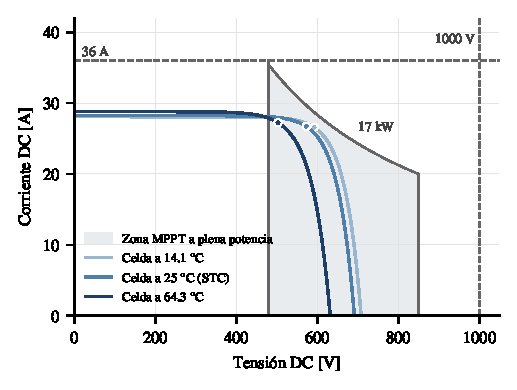
\includegraphics[width=0.92\anchofig]{soa.pdf}
\caption{Área de operación segura de un MPPT con dos cadenas de 17 módulos y curvas I--V aproximadas a \SI{1000}{W/m^2}. Los puntos marcan la máxima potencia.}
\label{fig:soa}
\end{figure}

\subsection{Estimación energética esperada}

La Tabla~\ref{tab:produccion} y la Fig.~\ref{fig:produccion} presentan la generación mensual calculada con \eqref{eq:efv} para \SI{168.3}{kWp}, con las HSP sobre el plano a \SI{10}{\degree} y el $PR$ de cada mes. El sistema generaría \SI{219.5}{MWh} al año, el 98.4\,\% del consumo anual, con un rendimiento de
\begin{equation}
\gamma_{fv} = \frac{E_{fv}}{P_{fv}} = \frac{\SI{219524}{kWh}}{\SI{168.3}{kWp}} = \SI{1304}{kWh/kWp}.
\end{equation}
La mayor generación ocurre en marzo y la menor en noviembre. De enero a abril y en setiembre la generación supera el consumo del mes, mientras que en los demás meses es menor. La energía consumida directamente, la depositada y la devuelta por la red se presentan en la Sección~\ref{sec:economia}.

\begin{table}[!t]
\caption{Pérdida por temperatura ($p_T$), factor de rendimiento, generación mensual estimada (\SI{168.3}{kWp}) y consumo}
\label{tab:produccion}
\centering
\footnotesize
\setlength{\tabcolsep}{2.5pt}
\begin{tabular}{l S[table-format=1.2] S[table-format=1.1] S[table-format=1.3] S[table-format=6.0] S[table-format=6.0] S[table-format=3.1]}
\toprule
{Mes} & {HSP} & {$p_T$ [\%]} & {$PR$} & {$E_{fv}$ [kWh]} & {Cons. [kWh]} & {$E_{fv}$/Cons. [\%]} \\
\midrule
Ene & 4.79 & 7.6 & 0.804 & 20092 & 18482 & 108.7 \\
Feb & 5.30 & 7.8 & 0.803 & 20066 & 17626 & 113.8 \\
Mar & 5.35 & 8.0 & 0.802 & 22395 & 18238 & 122.8 \\
Abr & 4.72 & 8.1 & 0.801 & 19094 & 18850 & 101.3 \\
May & 4.13 & 8.0 & 0.801 & 17262 & 19339 & 89.3 \\
Jun & 4.04 & 7.9 & 0.802 & 16378 & 18482 & 88.6 \\
Jul & 3.97 & 7.8 & 0.803 & 16613 & 18972 & 87.6 \\
Ago & 4.21 & 7.8 & 0.803 & 17638 & 19094 & 92.4 \\
Set & 4.51 & 7.8 & 0.803 & 18305 & 18238 & 100.4 \\
Oct & 4.19 & 7.7 & 0.804 & 17558 & 18727 & 93.8 \\
Nov & 3.90 & 7.7 & 0.804 & 15827 & 17993 & 88.0 \\
Dic & 4.36 & 7.7 & 0.804 & 18296 & 18972 & 96.4 \\
\midrule
Total & {--} & {--} & 0.803 & 219524 & 223013 & 98.4 \\
\bottomrule
\end{tabular}
\end{table}

\begin{figure}[!t]
\centering
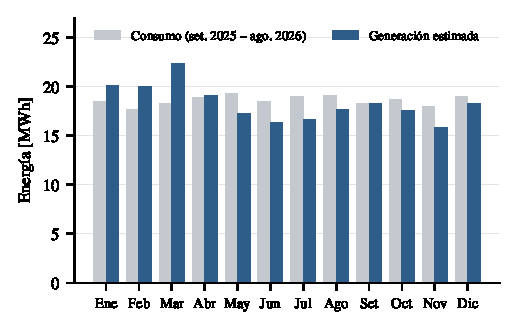
\includegraphics[width=0.92\anchofig]{produccion.pdf}
\caption{Consumo mensual del establecimiento y generación mensual estimada del sistema de \SI{168.3}{kWp}.}
\label{fig:produccion}
\end{figure}
